%%%%%%%%%%%%%%%%%%%%%%%%%%%%%%%%%%%%%%%%%%%%%%%%%%%%%%%%%%%%%%%%%
%%% %
%%% % weiiszablon.tex
%%% % The Faculty of Electrical and Computer Engineering
%%% % Rzeszow University Of Technology diploma thesis Template
%%% % Szablon pracy dyplomowej Wydziału Elektrotechniki 
%%% % i Informatyki PRz
%%% % June, 2015
%%%%%%%%%%%%%%%%%%%%%%%%%%%%%%%%%%%%%%%%%%%%%%%%%%%%%%%%%%%%%%%%%

\documentclass[12pt,twoside]{article}

\usepackage{weiiszablon}

\author{Kacper Rudź}

% np. EF-123456, EN-654321, ...
\studentID{EF-16045}

\title{Porównanie silników Unreal Engine i Unity pod kątem tworzenia gier}
\titleEN{Comparison of Unreal Engine and Unity software for game development}


%%% wybierz rodzaj pracy wpisując jeden z poniższych numerów: ...
% 1 = inżynierska	% BSc
% 2 = magisterska	% MSc
% 3 = doktorska		% PhD
%%% na miejsce zera w linijce poniżej
\newcommand{\rodzajPracyNo}{2}


%%% promotor
\supervisor{dr inż. Sławomir Samolej prof. PRz}
%% przykład: dr hab. inż. Józef Nowak, prof. PRz

%%% promotor ze stopniami naukowymi po angielsku
\supervisorEN{ PhD Eng Sławomir Samolej}

\abstract{Treść streszczenia po polsku}
\abstractEN{Treść streszczenia po angielsku}

\begin{document}

% strona tytułowa
\maketitle

\blankpage

% spis treści
\tableofcontents

\clearpage
\blankpage


\section*{Wykaz symboli, oznaczeń i skrótów (opcjonalny)}
\addcontentsline{toc}{section}{Wykaz symboli, oznaczeń i skrótów (opcjonalny)}%

1 $\div$ 2 stron wykaz ważniejszych symboli i oznaczeń (jeśli jest potrzebny).
\clearpage

\section{Wstęp}
%1 $\div$ 5 stron charakterystyka problematyki w świetle aktualnego stanu wiedzy
%i~techniki, ze wskazaniem na zagadnienia istotne z punktu widzenia realizowanej
%pracy. Na trzeciej stronie można zamieścić podziękowania dla osób, które
%przyczyniły się do powstania pracy dyplomowej. Na kolejnej stronie nieparzystej
%rozpoczyna się spis treści. Po spisie treści zalecane jest umieszczenie wykazu
%użytych symboli, oznaczeń i akronimów. Od tego miejsca rozpoczyna się numeracja
%rozdziałów. Na następnej stronie umieszcza się wprowadzenie do pracy
%(scharakteryzowanie problematyki pracy, uzasadnienie wyboru tematyki) oraz
%przedstawia: cel i/lub tezę pracy, zakres pracy, przyjęte założenia itp.
%Ostatni akapit wstępu musi zawierać zwięzłe sformułowanie celu i zakresu pracy. 

Silniki graficzne są technologią, która rozwijała się bardzo szybko. Pierwsze
gry, które używały silników graficznych z trójwymiarową grafiką pojawiły się w
drugiej połowie lat 90 ubiegłego wieku. Wcześniej silniki graficzne były używane
w branży filmowej w celu stworzenia prostych efektów specjalnych. Silniki
graficzne w tamtych czasach były bardzo proste i nie pozwalały na wiele. Zwykle
ograniczeniem były możliwości obliczeniowe komputerów graczy. Drużyny tworzące
gry zwykle składały się z kilkunastu osób, a budżety gier były małe w porównaniu
do budżetów branży filmowej. 

Wraz z biegiem czasu rozwój silników graficznych przyśpieszał, do czego
przyczynił się rozwój procesorów oraz kart graficznych. Z każdym rokiem silniki
graficzne były coraz bardziej zaawansowane i pozwalały na obsługę tekstur
większej rozdzielczości, wyższej jakości efektów cząsteczkowych, ulepszono
oświetlenie wprowadzając oświetlenie globalne czy ray tracing. Równolegle
rozwijały się techniki animacji szkieletowych oraz programy do modelowania,
teksturowania oraz animowania. W tym całym procesie nie zapomniano o poprawianiu
wydajności bibliotek graficznych co przełożyło się na wydajność silników
graficznych, które na nich operowały. 

Rozwój grafiki komputerowej musiał spowolnić po pewnym czasie. Już w roku
2016 pewne gry takie jak ‘Wiedźmin 3’ studia CD projekt Red, czy ‘Forza Horizon
3’ studia Playground Games były uznawane za bliskie fotorealizmu. Jednak za
najbardziej realistyczną grę pod względem grafiki jest gra ‘Red Dead Redemption
2’ studia Rockstar Games z roku 2018. 

W między czasie firmy tworzące gry rosły. Powstawały nowe studia, a inne były
wchłaniane przez największe korporacje, ale nadal powstawały gry tworzone przez
małe grupy osób. Aktualnie zespoły tworzące gry można podzielić na kilka grup: 

\begin {itemize}

\item Niezależni twórcy -- jedna lub kilka osób tworzy gry i wydaje je
zwykle samodzielnie. Często korzystają z gotowych silników graficznych lub
używają swoich bardzo prostych silników. Gry wykonane przez twórców
niezależnych: Factorio, Stardew Valley i pierwsze wersje gry Minecraft

\item Małe studia gier -- niewielkie firmy zatrudniające do kilkunastu
osób. Skończony produkt jest wydawany z pomocą wydawcy, rzadko samodzielnie.
Bardzo rzadko te firmy korzystają z własnych silników graficznych. Przykładowe
gry zrobione przez małe studia: Celeste, Ori and The Blind forest, Terraria

\item Średnie studia gier -- już większe firmy zatrudniające nawet
kilkaset osób. W przeszłości spora część korzystała z własnych silników
graficznych. Przykładowymi grami stworzonymi przez średnie studia są: Biomutant,
Baldurs Gate 3.

\item Duże i bardzo duże studia gier -- posiadają nawet do kilku
tysięcy pracowników. Bardzo często tworzą gry na własnych silnikach graficznych.
Studia takie potrafią pracować nad kilkoma grami jednocześnie. Przykładowe gry
stworzone przez duże studia: Wiedźmin 3 Dziki Gon, gry serii Far Cry i Assassins
Creed. 

\end{itemize} 

Większość twórców używa własnych silników graficznych lub silników komercyjnych
– do modelowania, animacji i teksturowania zwykle są używane narzędzia dostępne
na rynku. Małe studia i średnie studia bardzo rzadko używały własnych rozwiązań
i zwykle używały gotowych rozwiązań oferowanych przez firmy zajmujące się
tworzeniem i rozwojem silników graficznych. Duże studia posiadały własne silniki
graficzne, na których były tworzone gry. Jednak duże studia zaczynają przenosić
się na silniki innych twórców. Powodem takiej sytuacji jest koszt utrzymywania i
rozwoju własnych rozwiązań. 

Gry w dzisiejszych czasach są tworzone pod wiele platform. Platformą w tym
przypadku są rodziny systemów operacyjnych i konsole. Twórcy konsol co kilka lat
muszą wydać nowe konsole, ze względu na postęp technologiczny związany z
podzespołami. Zmiana jest na tyle spora, że wymaga znacznych zmian w systemach
operacyjnych konsol, co w konsekwencji ma wpływ na wydajność i stabilność gier.
Twórcy silników graficznych muszą aktualizować swoje silniki graficzne w celu
minimalizacji wpływu zmian na stabilność i wydajność gier. 



\clearpage

\section{Cel pracy}

Tematem pracy jest porównanie silników Unreal Engine i Unity pod kątem tworzenia
gier.  W tym celu należy wskazać różnice w budowie silnika. Zostały wskazane
różnice w pisaniu skryptów,  użyte języki programowania oraz różnice w
architekturze silników i różnice związane z kolejnością wykonywania metod i
funkcji. 


Ważnym elementem gier jest stabilność stworzonej aplikacji oraz ilość zasobów
wymaganych do prawidłowego funkcjonowania gry. W tym celu został przeprowadzony
test polegający na rozłożeniu w silniku kilku tysięcy kopii jednej postaci i
poruszaniu się kamery po ustalonej wcześniej ścieżce przez kilkadziesiąt minut.
Kopie postaci wykonują zapętlone animacje -- będzie 10 animacji i każda kopia
będzie wykonywała jedną z tych animacji. W trakcie testu zostały zebrane
informacje na temat ilości klatek na sekundę, zapotrzebowaniu na pamięć RAM oraz
pamięci VRAM i ile czasu w danej klatce aplikacja używała procesora i procesora
graficznego. Dane zostały zebrane z kilku różnych komputerów -- komputery
osobiste i laptopy -- o różnych specyfikacjach, a następnie dane zostały
przeanalizowane. Analizowane dane zostały ocenione pod względem różnych
kryteriów.



\clearpage


\section{Teoretycznie o silnikach graficznych}

Silniki graficzne nie są wymagane przy tworzeniu gier komputerowych, ale
znacząco przyśpieszają one proces twórczy. Częścią wspólną większości gier
komputerowych są dźwięk, elementy graficzne, takie jak modele, tekstury,
animacje, elementy interfejsu użytkownika oraz wszelkiego rodzaju skryptów i
sztucznej inteligencji. Dźwięk, animacje, modele i tekstury są opracowywane w
wyspecjalizowanych programach. 

Silniki graficzne są używane głównie przy tworzeniu modeli, animacji i tekstur
oraz jako solidna podstawa pod kod gry. Przykładowo program do grafiki
komputerowej 3D „Blender” posiada 3 silniki graficzne -- EEVEE, Cycles
i Workbench. Każdy z nich jest wyspecjalizowany w własnej dziedzinie – EEVEE
jako renderer casu rzeczywistego, Cycles jest używany do renderowania obrazów w
wysokiej jakości, Workbench jest używany do podglądów, modelowania i animacji.
Jako podstawę do kodu gry można użyć silnika graficznego podobnego do Unity lub
Unreal Engine. 

\subsection{Założenia silników graficzncyh używanych w grach}

Silniki graficzne używane w grach można podzielić na kilka większych
wyspecjalizowanych modułów \cite{GameEngineArchitecture}:
\begin{itemize}
\item Moduł obsługi urządzeń wejścia -- problemem urządzeń wejścia jest
ich różnorodność. Jest wiele urządzeń, dzięki którym można sterować postaciami w
grach, a jednymi z najczęściej używanych są klawiatury, myszki oraz pady. Poza
tym są jeszcze touchpady, czujniki pokroju żyroskopów i wiele innych. Zadaniem
tego modułu jest udostępnienie API, które pozwoli w prosty sposób oprogramować
przetwarzanie wejść. Wczytywanie danych z wejść może odbywać się na dwa różne
sposoby -- pollin jako statystyka ze zmiany wejść i przerwania jako
reakcja programu na zmianę stanu wejścia.

\item Matematyka -- matematyka w silnikach graficznych polega głównie
na optymalizacji obliczeń macierzy 4x4 lub 3x3, obliczeń związanych z wektorami
i kwaternionami. Macierze są wykorzystywane do reprezentacji transformacji
-- rotacja, skala i pozycja -- względem pewnego układu
odniesienia. Obliczenia wektorowe są potrzebne do obliczeń związanych z fizyką i
położeniem obiektu. Kwaterniony są używane zamiast macierzy transformacji, z
racji zjawiska gimbal lock, które polega na nałożeniu się na siebie osi rotacji.  

\item Fizyka -- moduł ten obejmuje głownie kinematykę. Zwykle fizyka
nie jest idealna i w swoich obliczeniach używa wielu uproszczeń. Jednak prawa
fizyki działające na obiekt w grze powinny być edytowalne -- zmiana
parametrów takich jak tarcie, prędkość, przyśpieszenie, prędkość odśrodkowa itp.
Jako obliczenia fizyczne zalicza się również kolizje. Kolizje powinny być
zdarzeniami i użytkownik silnika graficznego powinien mieć możliwość
wprowadzenia własnego kodu w odpowiedzi na zdarzenie. \cite{GameDevelpomenPhysics} 

\item Obsługa plików i tekstu – może wydawać się rzeczą banalną, jednak silniki
gra- ficzne używane do tworzenia gier powinny być w stanie obsługiwać różne
formaty plików oraz tekst. Głównymi formatami plików są formaty związane z
modelami graficznymi i teksturami – format fbx jest używany do wyeksportowania
modelu wraz z animacjami, png jest używany do przenoszenia tesktur. Obsługa
tekstu dotyczy obsługi różnych czcionek – systemowych, ale też dostarczanych
przez użytkownika silnika – różnych rozmiarów czcionek i innych właściwości,
które może ustawić użyt- kownik silnika graficznego
 

\item Obsługa elementów graficznych i rendering -- przez elementy graficzne
można rozumieć: elementy UI, wszelkiego rodzaju bryły wraz z animacjami, efekty
cząsteczkowe i oświetlenie. Każdy z tych elementów musi zostać uwzględniony w
procesie renderingu. Bryły w silnikach graficznych składają się z trójkątów,
ponieważ każde dowolne 3 punkty w przestrzeni są współpłaszczyznowe.  Do
stworzenia trójkąta potrzeba współrzędnych trzech punktów. Poza tym na bryłę
mogą być nałożone tekstury – mapy koloru, normalnych itp. Każda bryła może być
pod wpływem zjawisk fizycznych zaimplementowanych w silniku. 

\item Udźwiękowienie -- silniki graficzne używane w grach powinny pozwalać na
dodanie dźwięku do gry. W tym celu sam silnik powinien obsługiwać różne formaty
plików dźwiękowych jak i codeki. Najbardziej powszechnymi rodzajami codeków są:
H.264/AVC, AVI, VP9 oraz HEVC (H.256). Dodatkowo silnik graficzny powinien
pozwalać na używanie dźwięków przestrzennych oraz dźwięki statyczne -- dźwięk,
który nie zmienia się w zależności od zmiany położenia gracza. Dźwięk
przestrzenny powinien zmieniać się w zależności od położenia gracza od źródła
dźwięku i ta zmiana powinna być odzwierciedlana w urządzeniach audio – o ile te
urządzenia obsługują tę funkcję. 

\item Narzędzia do debugowania i rozwoju -- nowoczesne komercyjne
silniki graficzne powinny dawać możliwość dodawania własnych narzędzi do
silnika. Często zdarza się, że szybciej jest stworzyć narzędzie, które zrobi
daną rzecz za twórcę, niż tworzenie rzeczy ręcznie. Silnik graficzny w tym celu
powinien udostępniać interfejs, który pozwoli na tworzenie takich narzędzi lub
modyfikowanie starych. Kolejną ważną rzeczą są możliwości debugowania kodu.
Wśród narzędzi do debugowania powinny się znaleźć narzędzia do sprawdzania
zużycia zasobów przez grę. Błędy i wycieki pamięci mogą się zdarzyć nawet
najbardziej wprawnym programistom nawet w językach, które teoretycznie temu
zapobiegają. Błędy w grach często są ciężkie do znalezienia przy testach
-- często jest to związane z niedopatrzeniami w obliczeniach
fizycznych. 

\end{itemize}

Twórca gier powinien mieć możliwość używania każdego modułu bez ograniczeń. W
ten sposób użytkownik silnika graficznego jest w stanie stworzyć grę będąc
ograniczonym tylko umiejętnościami. Przykładem używania wielu modułów
jednocześnie jest wpływanie przez zjawiska fizyczne na szkielet postaci. Taka
postać może wydawać dźwięki w pewncyh punktach animacji. Jest to jeden z wielu
przykładów użycia wielu różnych komponentów w tym samym czasie. Ważnym aspektem
jest udostępnienie możliwości nanoszenia zmian do wymienionych modułów silnika
graficznego przez twórców gier. 

\clearpage

\subsection{Architektura silnika Unity}

Unity Engine jest silnikiem stworzonym i rozwijanym od 2005 roku. Silnik
graficzny zdominował rynek małych, średnich gier, gier na telefon oraz jest
używany w symulacjach. W Unity do programowania skryptów używa się języka C\#,
ale istnieje możliwość pisania skryptów za pomocą `Visual Scripting`. Skrypty w silniku, które używają metod Unity muszą dziedziczyć z ‘Monobehaviur’ lub klas pochodnych. 

Unity posiada bardzo prostą strukturę, a sam silnik pozwala twórcom na
nadpisywanie tylko określonych metod, ale jest ich na tyle dużo, że nie wpływa
to na elastyczność silnika. Cały silnik jest podzielony na kilka
części\cite{Unity:Architecture}: 
\begin{itemize}
\item Scena – w Unity poziomy zostały nazwane scenami. Przy przejściu między
scenami obiekty na scenie są usuwane. Jedynym wyjątkiem od reguły jest użycie
metody ‘DontDestroyOnLoad()’, która sprawi, że obiekt zostanie przeniesiony
między scenami. Poza tym dane między poziomami mogą być przenoszone poprzez
zmienne globalne i pola statyczne.
\item Obiekt – obiekty są elementami, które można ustawić na scenie. W obiektach
znajdują się komponenty, które mogą mieć różne funkcje. Obiekt na scenie ma
podstawowe transformacje takie jak rotacja, skala i przesunięcie. Jeden obiekt
może mieć wiele obiektów potomków, które mogą dziedziczyć transformacje. 
\item Komponenty – komponentem w silniku Unity można podzielić na wiele
kategorii: Rigidbody, Collider, Script, Mesh Rendere, AudioSource, Light itp.
Każdy element ma swoją funkcję od odtwarzania dźwięku po sterowanie animacjami. 
\end{itemize}
W Unity funkcjonują tzw. ‘prefab'y’. Są to szablonowe obiekty, które można
umieścić na mapie lub w skrypcie. Jest to mechanika pozwalająca poprzez zmianę
szablonu zmienić wszystkie elementy w silniku. Szablony obiektów mogą być bardzo
złożone i mogą korzystać z innych obiektów szablonów. Ich stosowanie bardzo
przyśpiesza proces tworzenia gier i pozwala na płynną naprawę błędów. W silniku
funkcjonuje system pozwalający na wywoływanie metod po pewnym czasie nazwany
‘Coroutine’. Mechanizm ten pozwala na odroczenie wykonywania kodu po pewnym
czasie lub później w danej klatce. Odroczenie zaczyna się zwykle słowem
kluczowym ‘yield’.  

Kolejnym aspektem, który należy przedstawić w Unity jest ‘Unity Flowchart’,
który przedstawia w jakiej kolejności są wywoływane metody w komponentach i
skryptach w silniku. Jest to mechanizm bardzo ważny, ponieważ pozwala
programiście na ustalenie kolejności wykonywania programu. Na rysunku
\ref{Unity:FlowchartFIG} przedstawiono kolejność wykonywania działań w silniku
Unity. Metody i funkcje zostały podzielone na 3 kategorie:

\begin{itemize}
    \item Metody i funkcje nadpisywalne przez programistę oznaczono kolorem białym
    \item Funkcje wewnętrzne zaznaczone kolorem szarym z zaokrąglonymi rogami
    \item Funkcje wewnętrzne wielowątkowe zaznaczone kolorem szarym z ostrymi
    rogami
\end{itemize}

Życie obiektu zostało podzielone na kilka etapów:
\begin{itemize}
\item Inicjalizacja – grupa metod, które są wywoływane, gdy obiekt zostanie
zainicjalizowany, wzbudzony lub zresetowany.
\item Fizyka – metody odpowiedzialne za obliczenia związane z fizyką oraz
animacjami, które są zależne od fizyki. Blok został podzielony na dwa mniejsze
bloki. W pierwszym bloku komponent animacji przetwarza przejścia miedzy
animacjami. W drugim bloku są obliczane transformacje kości animacji
szkieletowych. Między blokami zachodzi proces przeprowadzania obliczeń
fizycznych związanych z kinematyką. Etap zakończony jest metodami związanymi z
kolizjami oraz metodą, gdzie jest odroczona metoda ‘FixedUpdate’. Pętla fizyczna
może zostać wywołana kilka razy w trakcie jednej klatki. 
\item Zdarzenia wejścia – w tym etapie wywoływane są metody, które odpowiadają
za zdarzenia wciśnięcia klawiszy lub ruchu myszą. 
\item Logika Gry – pierwszą metodą w tym etapie życia obiektu jest metoda
‘Update’, która jest najczęściej używana do prostych obliczeń logiki gry.
Następnie są wywoływane metody, które zostały odroczone. Następnie w etapie jest
umieszczony blok odpowiedzialny za aktualizację animacji – zmiana stanów,
uruchomienie wydarzeń w trakcie animacji i przeprowadzenie animacji. Na końcu
etapu znajduje się metoda ‘LateUpdate’
\item Render Sceny – pierwszy etap generacji klatki. Grupa metod zawartych w tym
etapie służy głownie do wprowadzenia efektów graficznych.
\item Render interfejsu użytkownika i debugowania – interfejs użytkownika musi
być generowany po reszcie obiektów, aby był widoczny. Dodatkowo przed
interfejsem użytkownika są generowane efekty stworzone przez narzędzia
debugowania. 
\item Zakończenie i wstrzymanie klatki 0 w tym etapie znajduje się dwie metody.
Jedna z nich jest korutyną w silniku unity, która wznawia działanie na koniec
klatki. Druga metoda jest wywoływana tylko wtedy, gdy w silnku zajdzie zdarzenie
‘Pauza’.
\item Likwidacja obiektu – grupa metod, która jest wywoływana, gdy obiekt został
wstrzymany, obiekt został usunięty lub aplikacja została wyłączona. 
\end{itemize}

Każdy etap jest ważny jednak z widzenia programisty należy zastanowić się nad
funkcjami poszczególnych bloków, które można nadpisać. Pierwszym etapem jest
inicjalizacja, w której znajdują się metody:
\begin{itemize}
\item Awake() – metoda wywoływana, przy stworzeniu obiektu lub komponentu.
Metoda nie zostanie wywołana, kiedy obiekt nie jest ‘przebudzony’. Metoda może
zostać wywołana tylko raz.
\item OnEnable() – w przeciwieństwie do ‘Awake’ metoda może być wywoływana wiele
razy w trakcie życia obiektu lub komponentu, kiedy pole ‘enabled’ zmienia
wartość z ‘false’ na ‘true’.
\item Start() – metoda wywoływana tylko raz w czasie życia obiektu lub metody.
Jest ostatnią metodą w etapie inicjalizacji obiektu. 
\end{itemize}
Kolejną rzeczą niewspomnianą w silniku Unity jest konstruktor z języka C\#. Jest
on wywołany w trakcie tworzenia obiektu przed metodą ‘Awake’. Kolejnym etapem
życia obiektu w silniku unity jest pętla fizyczna. W niej znajdują się
następujące bloki: 
\begin{itemize}
\item FixedUpdate() – pierwsza metoda w pętli fizycznej, która pozwala na
stworzenie własnego kodu, który będzie używał części silnika odpowiedzialnego za
fizykę. Przykładem użycia może być zmiana prędkości obiektu w taki sposób, aby
ten orbitował wokół innego obiektu. 
\item Internal physics update – w tym momencie silnik przeprowadza obliczenia
fizyczne dla wszystkich aktywnych obiektów i komponentów. W tym czasie obliczane
są kolizje, dla których metody zostaną wywołane. 
\item OnTrigger – zdarzenie w silniku unity podczas kolizji ‘collider-trigger’. 
\item OnCollision – zdarzenie w silniku unity podczas kolizji typu
‘collider-collider’
\item yield Wait on FixedUpdate – kontynuacja działania metody ‘FixedUpdate’ po
jej odroczeniu
\end{itemize}
W trakcie pętli fizycznej znajdują się dwa duże bloki, które są używane w
animacjach. W tych blokach znajdują się następujące metody:
\begin{itemize}
\item State machine update – silnik przeprowadza aktualizacje maszyny stanów dla
kontrolerów animacji. Zmiana stanów maszyn jest przeprowadzana wielowątkowo. 
\item OnStateMachine Ender/Exit – metody wywoływane podczas zmiany stanów w
maszynie stanów. Pozwala programistom na wprowadzenie własnego kodu.
\item ProcessGraph – blok odpowiedzialny za przetworzenia grafów używanych w
animatorze. Obliczany jest czas, w jakim zajdzie przejście między klatkami
animacji. W tym czasie mogą znajdować się wcześniej zdefiniowane zdarzenia, co
musi zostać wywołane. 
\item Fire animation events - animacje mogą posiadać zdarzenia, które wywołują
konkretną metodę skryptu w wybranym momencie. 
\item StateMachineBehaviour callbacks - dotyczy metod wywoływanych w trakcie
przejścia między stanami. 
\item OnAnimationMove – metoda wywołana w przypadku ruchu obiektu na bazie
animacji. Ruch ten nazwano ‘Root Motion’, gdzie ‘Root’ oznacza nazwę kości,
która odpowiada za pozycję całego obiektu.  
\item ProcessAnimation –
\item OnanimationIK
\item WriteProperties
\end{itemize}





\begin{figure}[ht]
    \centering
    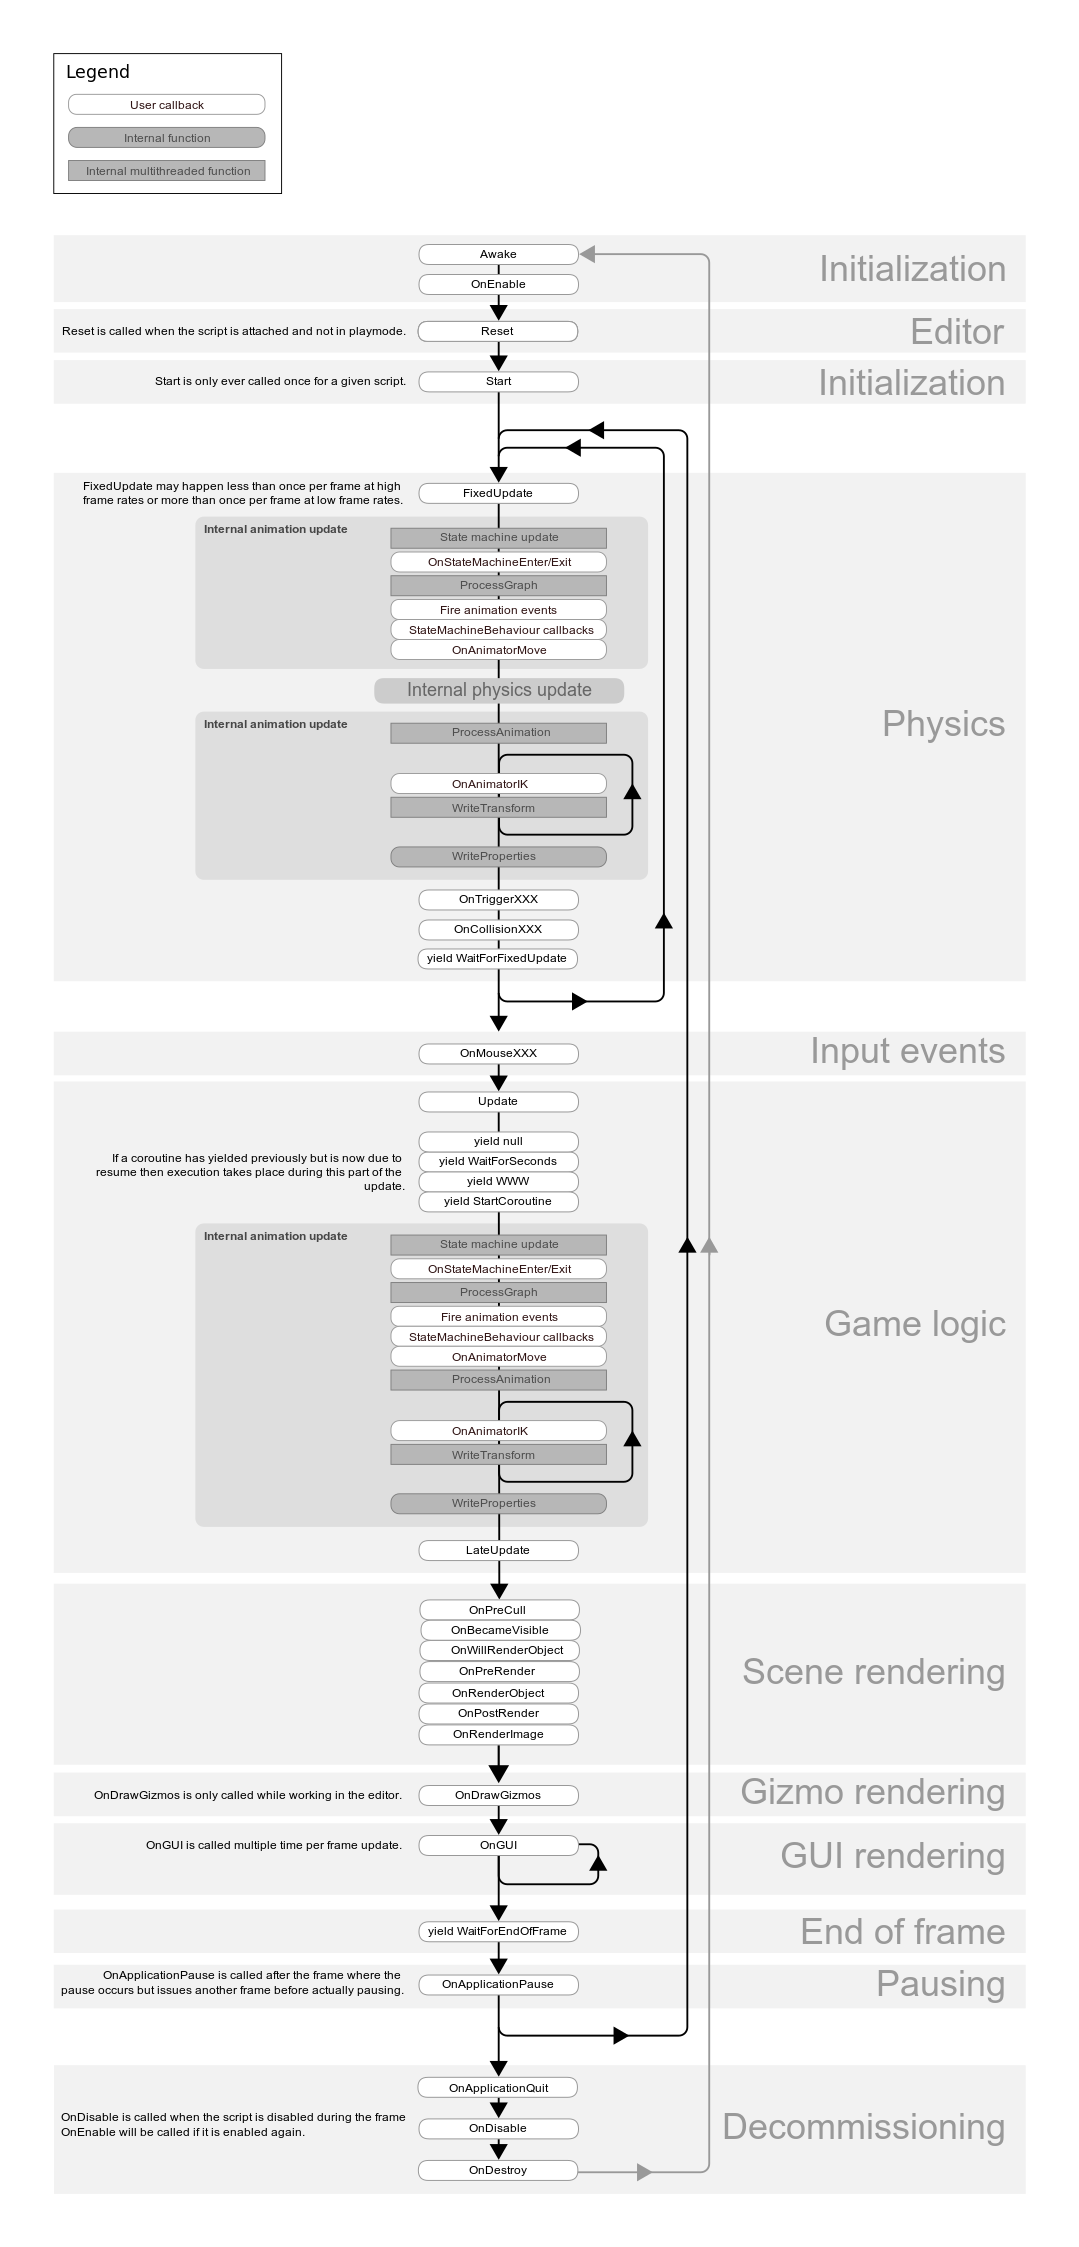
\includegraphics[width=10.5cm]{figures/UnityFlowchart.png}
    \caption{Unity Flowchart\cite{Unity:Flowchart}}
    \label{Unity:FlowchartFIG}
\end{figure}

\clearpage
\subsection{Architektura silnika Unreal Engine}
Silnik Unreal Engine jest powstałym w 1991 roku rozwijanym do dzisiaj. Silnik
aktualnie jest jednym z najbardziej rozwiniętych silników graficznych. W silniku
można pisać kod na dwa sposoby: 
\begin{itemize}
\item Kod c++ -- Unreal Engine posiada możliwość pisania kodu za pomocą języka
c++. W tym przypadku twórca może tworzyć własne klasy za pomocą dziedziczeniu z
klas zaimplementowanych w silniku. Gry tworzone w ten sposób będą działać
szybciej niż te napisane za pomocą „Blueprint`ów” kosztem dłuższego czasu kompilacji. 
\item Blueprint`y -- jest to programowanie obiektowe za pomocą bloków.
Programowanie w ten sposób działa podobnie do programowania za pomocą c++ -- jest
obsługiwane tworzenie programistycznych interfejsów, dziedziczenie i
przysłanianie metod. Zaletą tego rozwiązania jest szybkikrótki czas kompilacji.
\end{itemize}

Twórcy silnika Unreal Engine nie narzucają w jaki sposób należy używać ich
narzędzia. Obie metody programowania są ze sobą kompatybilne i można ich używać
naprzemiennie. Cały silnik jest bardzo plastyczny i jasno podzielony na wiele
klas, które można nadpisać. \cite{UnrealEngineArchitecture}. 

Silnik został podzielony na 4470 różnych klas, które można nadpisać i dowolnie
używać, ale najczęściej używane to:
\begin{itemize}
\item GameInstance –- Istnieje tylko jedna instancja tej klasy w całym silniku,
która działa od rozpoczęcia programu do jego wyłączenia. Obiekt klasy może być
użyty w celu przechowywania danych między poziomami, zapisywania i wczytywania
danych np. zapisu gry lub ustawień gracza oraz do przechowywania funkcji, które
muszą być dostępne globalnie. 

\item GameMode –- Klasa, która definiuje logikę w danym trybie gry. W grze może
być zaimplementowanych wiele trybów, ale tylko jeden obiekt typu GameMode może
istnieć. Obiekt tej klasy jest zawarty w obiekcie GameInstance. GameMode jest
odpowiedzialny za obsługę wejścia, kolizji oraz zmian poziomów, stworzenie
obiektu gracza i systemy zarządzania punktami. Zwykle każdy poziom ma swój
obiekt typu GameMode. 

\item GameState –- klasa używana do przechowywania i zarządzania danymi pokroju
obecne punkty, pozostały czas, zdrowie gracza i inne ważne dane gry. Obiekt jest
zwykle zarządzany przez obiekt GameMode i w przypadku gry sieciowej jest
replikowany z serwera do klientów. Obiekt tej klasy jest łatwo dostępny przez
inne obiekty w programie pokroju kontrolerów gracza i obiektów klasy Actor.
Najważniejszą funkcją obiektów tej klasy jest synchronizacja stanu gry dla
wszystkich graczy. 

\item LevelScriptActor –- specjalny typ aktora w silniku, który pozwala na
stworzenie logiki, która będzie wykonywana w czasie ładowania poziomu. Obiekt
klasy pozwala na ustawienie początkowego ustawienia klasy GameState, stworzenie
i ustawienie obiektów, aktywacja wydarzeń i wiele innych. Klasa jest nadpisywana
w celu stworzenia skryptów, które będą używane w zależności od poziomu. 

\item Controller –- kontrolery dzielą się na dwie kategorie: kontrolery AI i
kontrolery gracza. Te obiekty tej klasy są odpowiedzialne za przetwarzanie i
przekazanie sygnałów wejścia do kontrolowanego obietku. Kontorlery determinują
sposób nawigacji postaci przez poziom, reakcję postaci w różnych sytuacjach oraz
interakcje z innymi obiektami w poziomie. 


\item Pawn/Actor/Chracter -- Actor jest najbardziej podstawowym obiektem, który
można postawić na poziomie. W obiekcie tego typu znajdują się różne komponenty
typu oświetlenie, siatka czy kamera. Obiekty tego typu są bardzo proste i mogą
zostać użyte do implementacji własnych zachowań. Pawn jest klasą pochodną, która
posiada implementację złożonej fizyki, może oddziaływać na obiekty. Obiekty typu
Pawn są używane do stworzenia zachowań imitujących pojazdy lub zwierzęta.
Character jest klasą dziedziczącą z klasy Pawn. Obiekty klasy character w
porównaniu do dwóch poprzednich klas posiadają własną implementację ruchu,
komponentów animacji i zmiany wejścia na ruch fizyczny. Character jest klasą
używaną do stworzenia obiektu imitującego człowieka lub zwierzę. 

\item Komponenty –- komponentami w UnrealEngine są wszystkie klasy, które
dziedziczą z klasy UActorComponent, a jest ich ponad 400. Komponenty zwykle
odpowiadają za jedną funkcjonalność np. oświetlenie, kolizje, fizyka, kamera,
siatka itp.  W ten sposób w silniku został stworzony stopień modularności, który
pozwala na wysoką elastyczność i skalowalność projektu. Jeden komponent może
zostać użyty w wielu różnych klasach. Komponenty mogą zostać użyte tylko w
klasach dziedziczących z klasy Actor lub innych komponentach. KOlejną metodą jest 


\end{itemize}

Kolejną rzeczą, która jest ważna w programowaniu gier jest kolejność wykonywania
kolejnych części programu. W silniku Unreal każdy element jest inny i twórca
gier ma możliwość zmiany każdej części silnika. Poza tym silnik posiada wiele
metod, które są wspólne dla wielu elementów. Rysunek \ref{UE:ActorLifeCycle}
przedstawia cykl życia obiektu w silniku UnrealEngine. Na rysunku przedstawione
różne ścieżki. Jeżeli Aktor musiał być wczytany, ponieważ był częścią mapy, to
cykl życia zaczyna się od punktu `LoadMap`. Funkcja ‘AddToWorld’ jest częścią
działania ‘LoadMap’. Kolejnym ważnym punktem na tej ścieżce jest metoda
`PostLoad`, która jest wywoływana po wczytaniu mapy. 

Kolejną metodą jest `RouteActorInitialize`, który odpowiada za inicjalizacje
ścieżki poruszania się obiektu po świecie jeżeli została ustalona. Następnie
znajdują się 3 metody wywoływane podczas inicjalizacji komponentu. Powodem
stworzenia tych metod jest problem używania komponentów przez inne komponenty. W
`PreInitializeComponents` powinno się inicjalizować zmienne, tworzyć komponenty
i zmieniać ustawienia komponentu, który wywołał tę metodę.
`InitializeComponents` najczęściej jest używany podczas uzyskiwania dostępu do
innych komponentów. Ta metoda jest używana do uzyskania dostępu do innych
komponentów, punkcie czasu są one zainicjalizowane, ale nie można uzyskać
dostępu do niektórych pól. ‘PostInitializeComponents’ jest wywoływana jako
ostatni etap inicjalizacji. W tym momencie komponent skończył inicjalizację i
twórca kodu może w tym momencie wczytywać dane z innych komponentów należących
do tego samego pionka lub aktora bez błędu związanego z nieistnieniem obiektu.
Kolejną ważną i często używaną metodą jest metoda `BeginPlay`, która jest
wywoływana przed pierwszą klatką, kiedy dany pionek został stworzony lub po
wczytaniu poziomu. Metoda nie zostanie wywołana, jeżeli gra jest zapauzowana.
Przed omówieniem metody `Tick` należy opisać drogę od ‘SpawnActor’ i
‘SpawnActorDeffered’. Obie te ścieżki są podobne i główna różnica polega na
odroczeniu stworzenia obiektu. `SpawnActor` zacznie tworzyć aktora w momencie
wywołania metody `SpawnActor`. `SpawnActorDeffered` rozpocznie tworzyć obiekt po
pewnym czasie lub przy spełnieniu pewnych warunków. Konstruktor obiektu z języka
C++ zostanie wywołany dopiero w bloku `ExecuteConstruction`. W między czasie
jest wywołana metoda `OnConstruction` i `PostConstruction`. Metoda
`OnActorSpawned` zostaje wywołana po zakończeniu tworzenia obiektu. 

Najczęściej używaną metodą, która jest wywoływana co klatkę jest metoda ‘Tick’
na rysunku \ref{UE:ActorLifeCycle}. Tę metodę posiada każdy komponent i pionek
oraz każdy z tych obiektów może mieć wiele metod typu tick zgodnie z
dokumentacją \cite{UE:TickingActor}. Dodatkowo według tej samej dokumentacji te
metody mogą być wywoływane w różnym punkcie obliczeń silnika. W dokumentacji
wyróżniono 6 grup, kiedy metoda `Tick` może zostać wywołana, ale nie wszystko
zostało udokumentowane. Opisane grupy to:

\begin{itemize}
    


\item TG\_PrePhysics – pierwsza grupa, najczęściej odpowiada za aktualizację
stanu obiektów, na które wpływa fizyka, ale nie zmienia położenia, prędkości i
przyśpieszenia obiektów. Najlepszy moment na zebranie sygnałów wejściowych i
przekazanie ich do komponentów zajmujących się ruchem.

\item TG\_DuringPhysics – wszystkie komponenty używające kolizji lub fizyki muszą
zostać zaktualizowane. Obiekty znajdujące się w tej grupie obliczają kolizje i
inne elementy fizyczne. Twórcy gier mogą zmienić ustawienia silnika aby animacje
były aktualizowane w tej grupie. Obiekty w tej grupie mogą być aktualizowane
kilka razy w ciągu jednej iteracji pętli ze względu na możliwość implementacji
symulacji fizyki w silniku. 

\item TG\_PostPhysics – domyślnie do tej grupy należą wszystkie komponenty
zajmujące się animacjami, elementy interfejsu użytkownika i elementy graficzne. 

\item TG\_POostUpdateWork – do tej grupy powinny należeć obiekty, które wymagają
dużej ilości obliczeń lub nie są istotne z punktu widzenia działania gry.
Obiekty w tej grupie są aktualizowane rzadziej niż te w innych grupach, więc
jest to idealna grupa dla sztucznej itenligencji, która wymaga dużej ilości
obliczeń. 
\end{itemize}

Zakończenie cyklu życia aktora w silniku Unreal Engine może rozpocząć się w
kilku przypadkach:
\begin{itemize}
\item Wywołanie metody `Destroy` - ze względu na architekturę silnika,
programista go używający nie może zniszczyć obiektów dziedziczących z klas
komponentów lub klasy aktora nie mogą być zniszczone wywołaniem zwykłego
destruktora. Metoda `Destroy` najpierw bezpiecznie usunie obiekt z elementów
silnika, a następnie wywoła destruktor obiektu.
\item Czas życia Aktora się skończył – w trakcie działania gry tworzonych i
usuwanych jest wiele obiektów. W silniku zaimplementowano mechanizm, który
pozwala na usuwanie obiektów po jakimś czasie ustalonym przez twórcę gry. Czas
życia obiektu można ustawić za pomocą metody ‘SetLifeSpan(float time)’, która
rozpocznie niszczenie obiektu po czasie podanym w sekundach.
\item Zmiana poziomu – gry mogą się składać z wielu poziomów i zabezpieczenie
programu przed wyciekami pamięci przy zmianie poziomów jest bardzo ważną rzeczą.
Przy zmianie poziomów wszystkie obiekty w poziomie zostają zniszczone i zostaje
wczytany nowy poziom. 
\item Zakończenie gry w Edytorze – testowanie funkcji w edytorze jest ważnym
elementem tworzenia elementów gry w każdym silniku. Gra w edytorze może być
włączana nawet kilkaset razy, co bez usuwania obiektów może doprowadzić do
wycieku pamięci i w konsekwencji wyłączenie się edytora. 
\item Zakończenie gry – wywołane w przypadku zakończenia rundy, utraty
połączenia lub w przypadku osiągnięcia końca gry i wyświetlenia napisów
końcowych. 
\item Zakończenie programu 
\end{itemize}

Jeżeli jeden z tych warunków zostanie spełniony zostanie wywołana metoda
`EndPlay`. Metoda ma na celu zatrzymanie obiektu, zatrzymanie wywoływania metod
typu `Tick`, wysłanie sygnału o usuwaniu obiektu do obiektów `GameState`i innych
obiektów w grze. Obiekt zostanie oznaczony flagą `RI\_PendingKill`, co
zakolejkuje go do usunięcia za pomocą mechanizmu `Garabage Collector`. Przy
usuwaniu zostaną wywołane metody `BeginDestroy`, `IsReadyForFInishDestroy` i
`Finishdestroy`, w których powinna być zawarta implementacja usuwania elementów
alokowanych dynamicznie.  


\begin{figure}[ht]
    \centering
    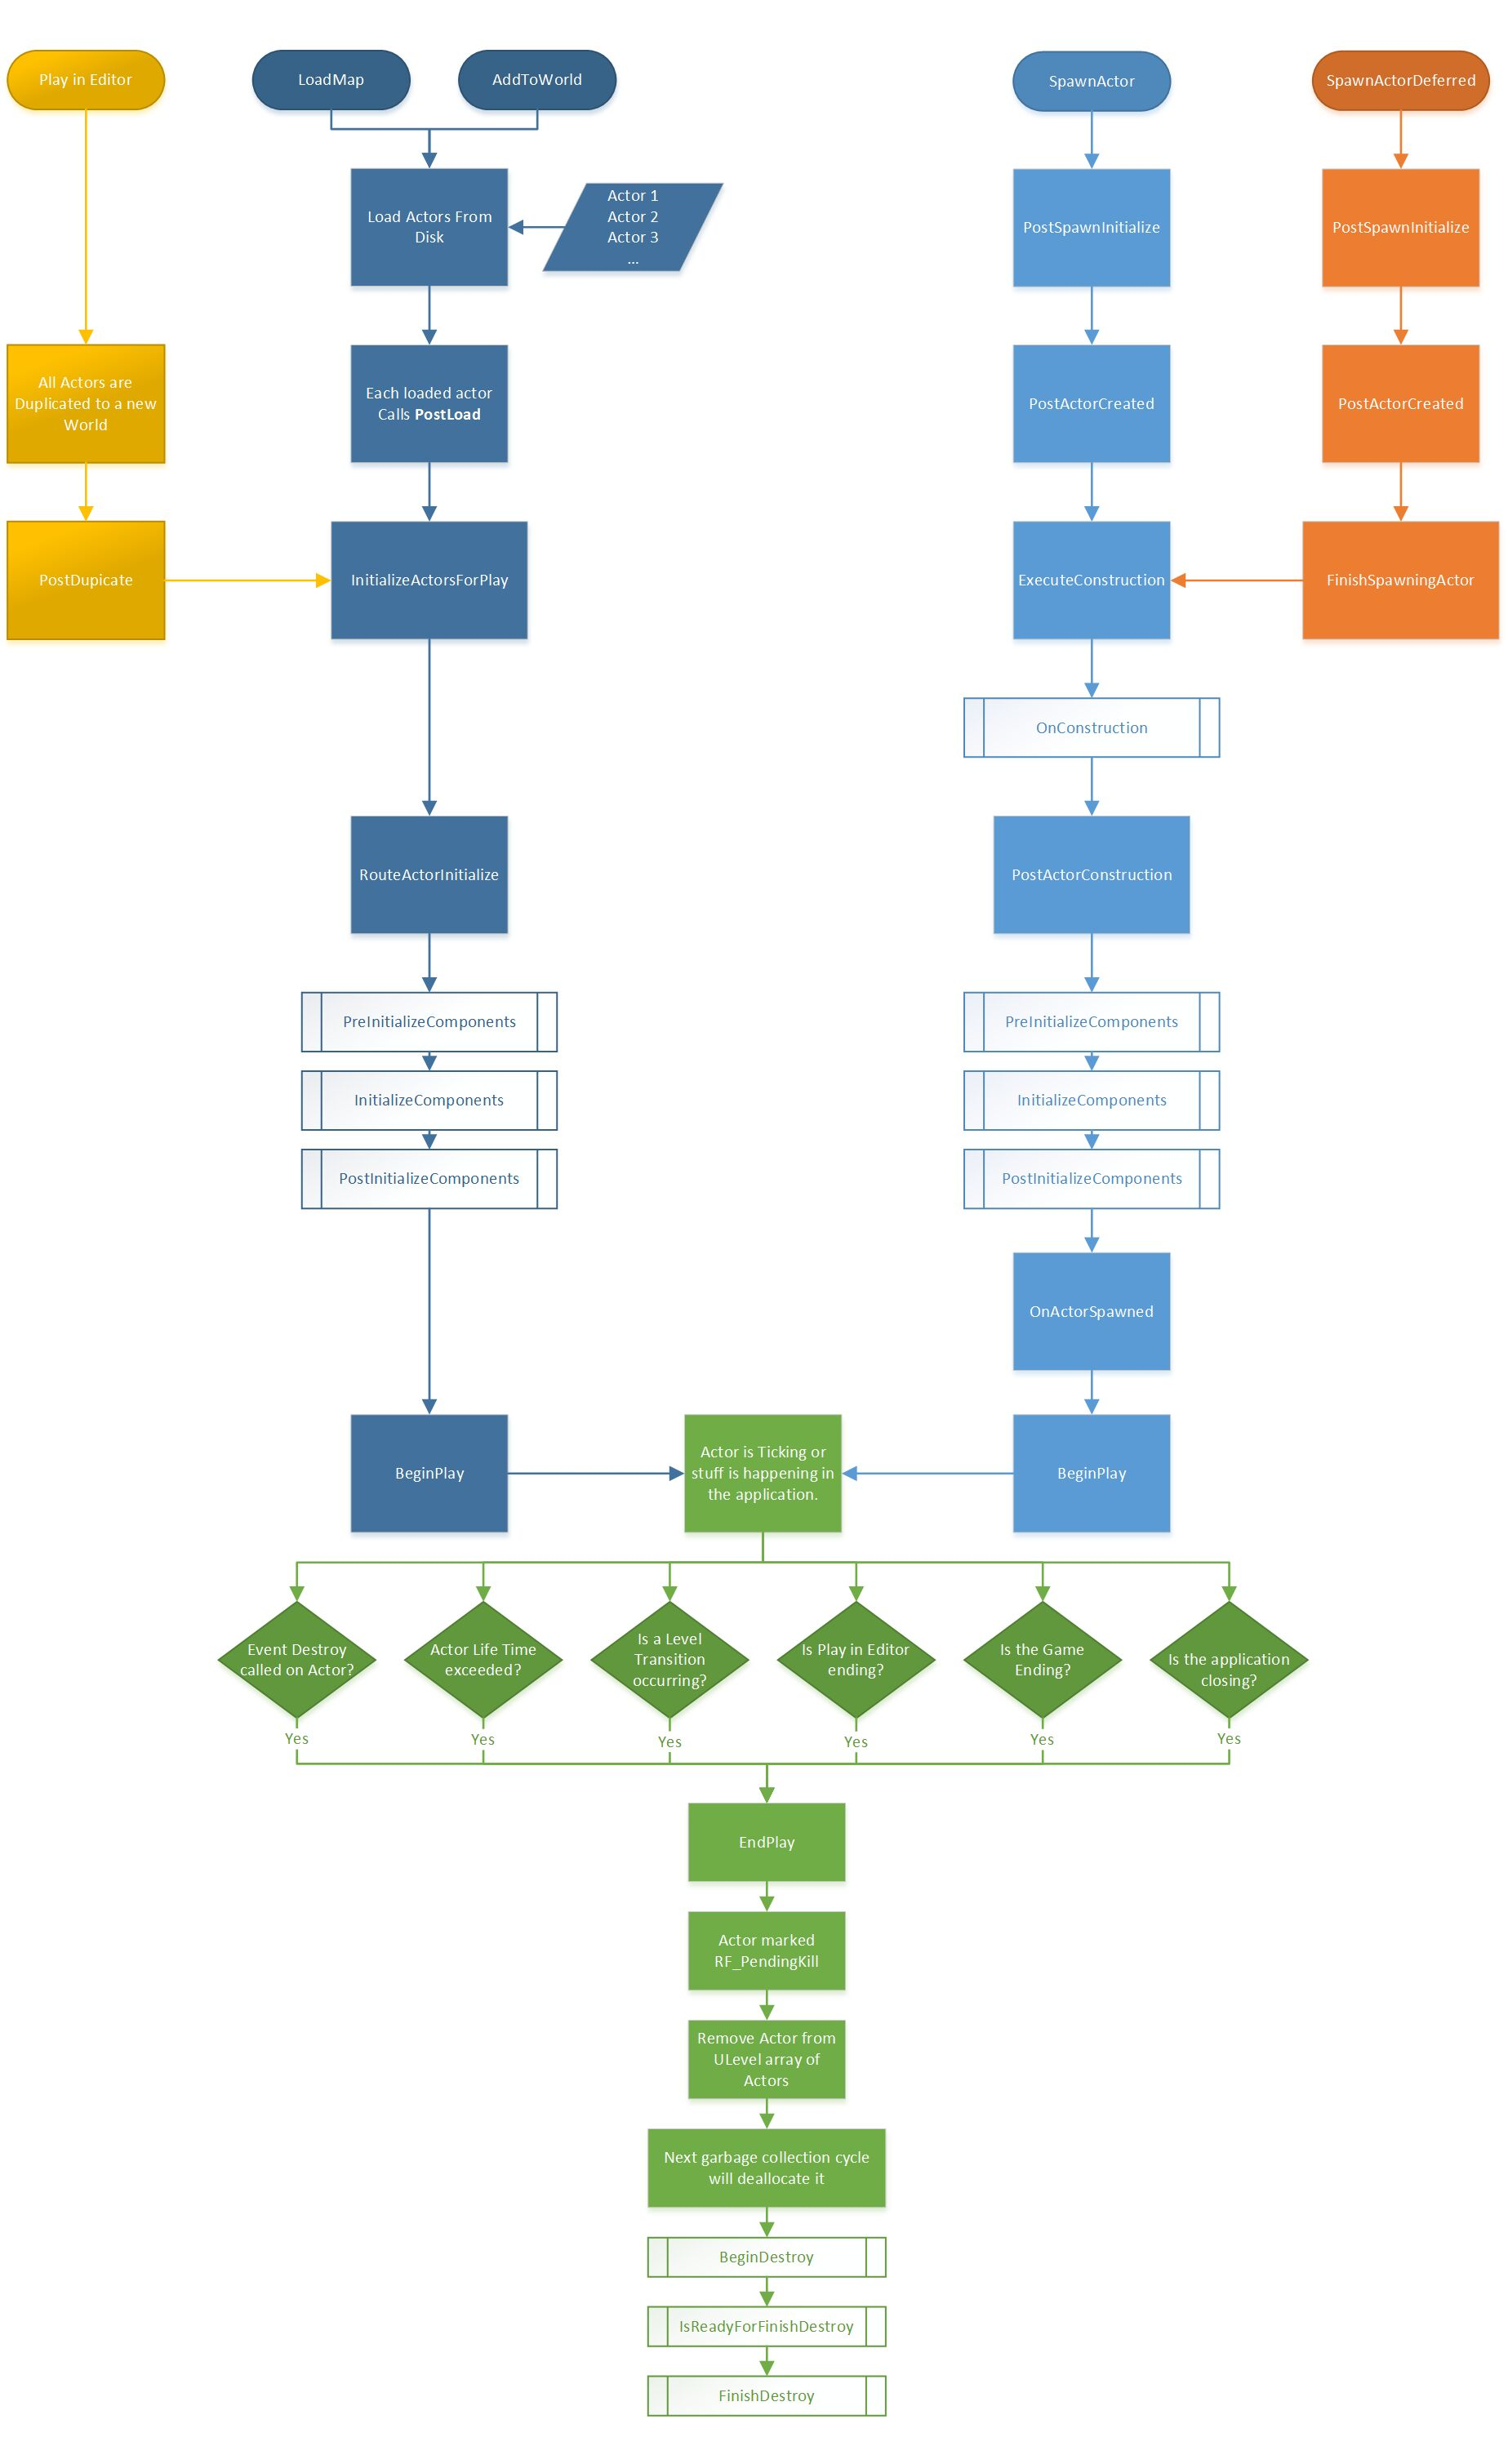
\includegraphics[width=14cm]{figures/ActorLifeCycle1UNREAL.jpg}
    \caption{Cykl życia obiektu w silniku Unreal Engine\cite{UE:ActorLifeCycleSource}}
    \label{UE:ActorLifeCycle}
\end{figure}





\clearpage
\subsection{Różnice między silnikami}



\clearpage	
\section{Testowanie wydajności silników Unity i Unreal Engine}

\subsection{Założenia i zakres  testów oraz klasyfikacja danych}
Głównym testem będzie sprawdzenie jak silniki radzą sobie z generacją obrazu w
czasie rzeczywistym, gdzie obiektów w grze jest kilka tysięcy. Ilość obiektów
będzie wyznaczona metodą prób i błędów w taki sposób, aby silniki graficzne
działały w przedziale <10-25> klatek na sekundę w pierwszych kilku sekundach
trwania testu. Obiekty będą prostymi modelami z zapętlonymi animacjami wybranymi
wcześniej w sposób losowy – rozstawienie, animacje i prędkość animacji zostaną
wygenerowane skryptem i będą takie same dla obu silników. Ruch kamery zostanie
zdefiniowany przed testem podobnie jak obiekty rozstawione w świecie. 

Głównym celem testów jest oszacowanie, który silnik graficzny lepiej radzi sobie
z generacją klatek w czasie rzeczywistym. Kryteriami będą:
\begin{itemize}
\item Licznik FPS – jest to wartość równa 1/(czas wykonania programu między
klatkami). Najważniejsze kryterium ze wszystkich, jednak różnica między 1-2
klatek na sekundę nie jest znacząca. Dodatkowo można określić stabilność
programu szukając ile razy wystąpiła znacząca fluktuacja od wartości średniej. 
\item Użycie czasów procesora i procesora graficznego – ważne kryterium, które
pomoże ustalić, który z silników graficznych wymaga większej mocy obliczeniowej.
Jest to drugorzędny znacznik jednak nie mniej ważny. 
\item Zużycie pamięci RAM i VRAM – pozostałe znaczące znaczniki przy ustalaniu
wydajności gry komputerowej mające wpływ na jakość obrazu i stabilność programu. 
\end{itemize}
Sprawdzana będzie nie tylko ilość używanych zasobów, ale też stabilność programu
i fluktuacje w zużyciu zasobów. 




\subsection{Program w unity}

\subsection{Program w Unreal Engine}

\clearpage
\section{Zbieranie i analiza danych}
Gry komputerowe trafiają na różne urządzenie z różną mocą obliczeniową.
Dodatkowo komputery posiadają wiele programów i usług działających w tle, które
mają wpływ na wynik testów. Te czynniki należy wziąć pod uwagę podczas trwania
testów. Gry komputerowe trafiają na różne urządzenie z różną mocą obliczeniową.
Dodatkowo komputery posiadają wiele programów i usług działających w tle, które
mają wpływ na wynik testów. Te czynniki należy wziąć pod uwagę podczas trwania
testów. Dlatego testy odbędą się na komputerach – komputerach stacjonarnych i
laptopach - z systemem Windows 10 lub Windows 11. System operacyjny został
wybrany ze względu na popularność wśród graczy. Gry komputerowe trafiają na
różne urządzenie z różną mocą obliczeniową. Dodatkowo komputery posiadają wiele
programów i usług działających w tle, które mają wpływ na wynik testów. Te
czynniki należy wziąć pod uwagę podczas trwania testów. Dlatego testy odbędą się
na komputerach – komputerach stacjonarnych i laptopach - z systemem Windows 10
lub Windows 11. System operacyjny został wybrany ze względu na popularność wśród
graczy. Zgodnie z badaniem z lutego 2024 roku wykonanym przez platformę Steam –
największa aplikacja, która pozwana na kupno i granie w gry na komputery
osobiste i laptopy – gracze używający ich sklepu korzystający z systemów Windows
10 i Windows 11 stanowią ok
96,15\% wszystkich graczy korzystających z komputerów – odpowiednio 54,19\% i 41,96\%. 

\begin{figure}[ht]
    \centering
    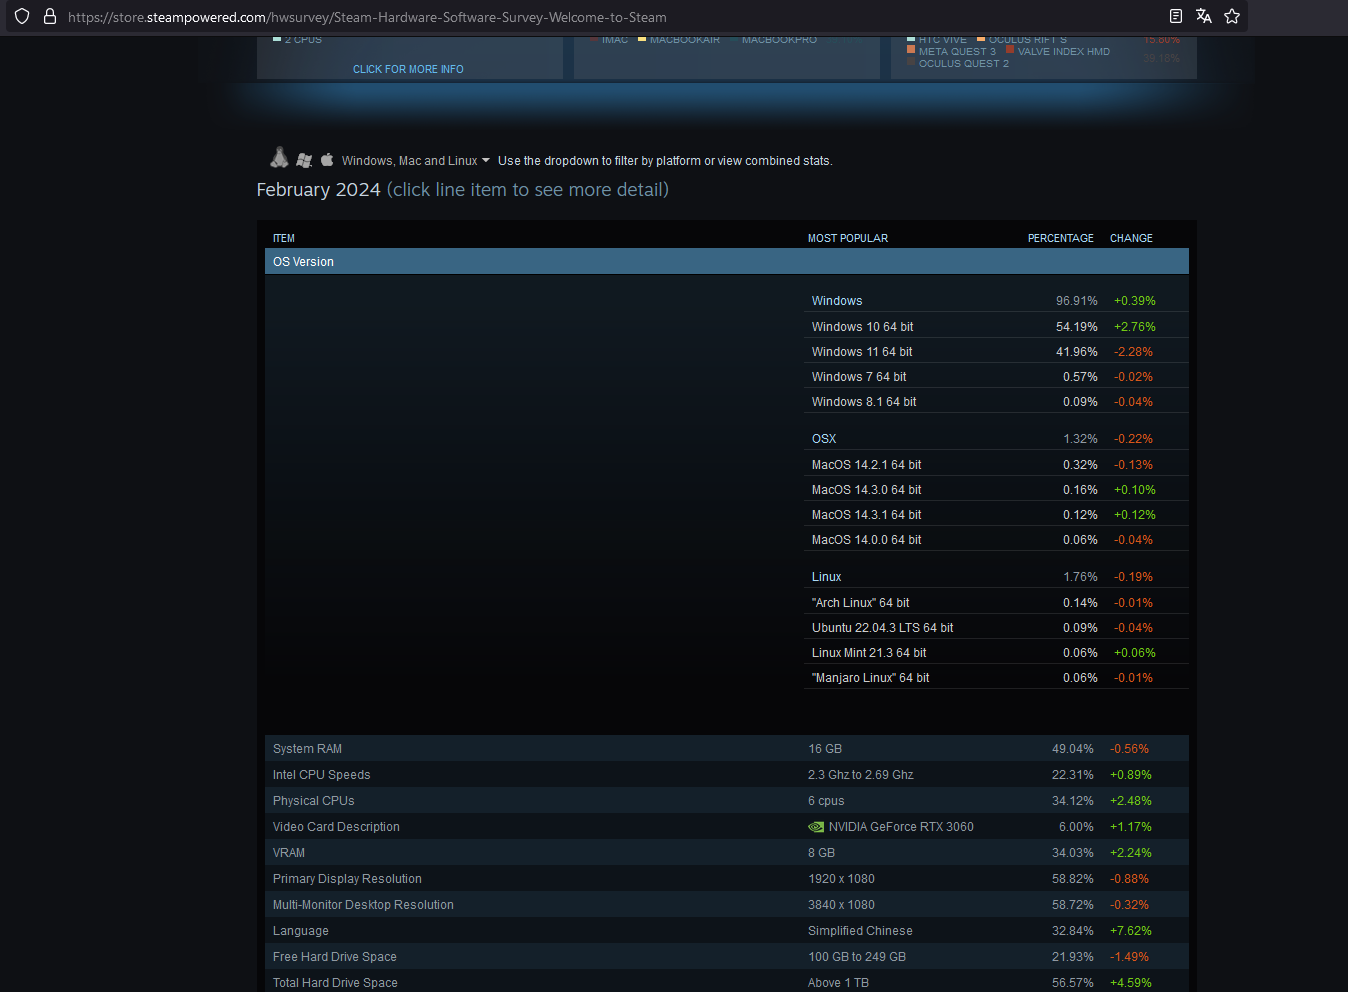
\includegraphics[width=14cm]{figures/SteamHardwareSoftwareSurvay.png}
    \caption{Statystyka użycia systemów operacyjnych przez graczy komputerowych przeprowadzona przez Steam \cite{SteamSurvey}}
    \label{SteamHardwareSoftwareSurvay}
\end{figure}

\clearpage
\section{Podsumowanie i wnioski}

\clearpage

\section*{Załączniki}
\addcontentsline{toc}{section}{Załączniki}



\clearpage

\addcontentsline{toc}{section}{Literatura}

\begin{thebibliography}{4}
\bibitem{GameEngineArchitecture} Jason Gregory: Game Engine Architecture, CRC Press 2019
\bibitem{GameDevelpomenPhysics} David M. Bourg, Bryan Bywalec: Physics for Game Development, O\'Reilly 2013

\bibitem{Unity:Architecture} https://docs.unity3d.com/Manual/CreatingGameplay.html Dostęp \today
\bibitem{Unity:Flowchart} https://docs.unity3d.com/Manual/ExecutionOrder.html Dostęp \today

\bibitem{UnrealEngineArchitecture} https://docs.unrealengine.com/4.26/en-US/ProgrammingAndScripting/ProgrammingWithCPP/UnrealArchitecture/ Dostęp: \today
\bibitem{UE:ActorLifeCycleSource} https://docs.unrealengine.com/4.27/en-US/ProgrammingAndScripting/ProgrammingWithCPP/UnrealArchitecture/Actors/ActorLifecycle/ Dostęp: \today
\bibitem{UE:TickingActor} https://docs.unrealengine.com/4.27/en-US/ProgrammingAndScripting/ProgrammingWithCPP/UnrealArchitecture/Actors/Ticking/ Dostęp \today

\bibitem{SteamSurvey} https://store.steampowered.com/hwsurvey/Steam-Hardware-Software-Survey-Welcome-to-Steam Dostęp: \today

\end{thebibliography}

\clearpage

\makesummary

\end{document} 
